\documentclass{article}
\usepackage[UTF8]{ctex}
\usepackage{amsmath}
\usepackage{amssymb}
\usepackage{graphicx}
\usepackage{float}
\usepackage{datetime}
\usepackage{geometry}

\geometry{a4paper, top=2.54cm, bottom=2.54cm, left=3.18cm, right=3.18cm}

\author{刘思昀 SLST 2022522011}

\title{General Physics II 用惠斯通电桥测电阻}

\begin{document}

\date{\formatdate{8}{5}{2024}}

\maketitle

\section{惠斯通桥测量电阻}
用万用表粗测待测电阻,测得$R_x=0.50248 k\Omega = 502.48\Omega$

连接惠斯通桥电路后,$U_{AC} = 3.0 V$,选取5个不同的$R_1 / R_2$比值,分别调节电阻箱阻值使电桥平衡,电阻箱阻值读数记为$R$,电压表示数此时最接近于0,记为$U$;改变电阻箱阻值,使得电压表示数发生微小变化,此时电阻箱阻值记为$R'$,电压表示数记为$U'$。最后计算$R_x$和电桥灵敏度$S$。

其中,
\begin{align*}
    R_x &= R \cdot \frac{R_1}{R_2} \\
    \Delta R &= R' - R \\
    \Delta U_0 &= U' - U \\
    S &= \lvert \frac{\Delta U_0}{\frac{\Delta R}{R}} \rvert
\end{align*}

\begin{figure*}[htbp]
    \centering
    
\includegraphics[width=1.0\textwidth]{1-1.png}
    \caption{惠斯通桥测量电阻}
\end{figure*}

对于5次结果平均值,得到$R_x = 503.2 \Omega, S = 0.485$

对比粗测结果,相差
\begin{equation*}
    \delta = \frac{503.2 - 502.48}{502.48} \times 100 \% = 0.143 \%
\end{equation*}

\begin{figure*}[htbp]
    \centering
    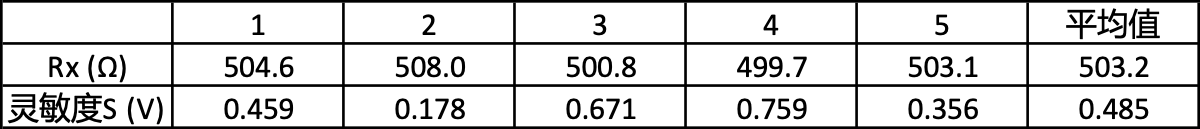
\includegraphics[width=1.0\textwidth]{1-2.png}
    \caption{平均测量结果}
\end{figure*}

\section{惠斯通电桥灵敏度与电桥端电压的关系}
分别选取$U_{AC} = 1.0 V, 3.0 V, 5.0 V, 7.0 V, 9.0 V, R_1 = 2000 \Omega, R_2 = 2000 \Omega$,调节电桥至平衡状态时,电阻箱阻值$R = 504.5 \Omega$,故实验中保持电桥桥臂电阻比值$R/R_2 = 0.2522$和电桥桥臂电阻总值$R_1 + R_2 + R + R_x = 5007.7 \Omega$不变。

改变电阻箱阻值,使得电压表示数发生微小变化,此时电阻箱阻值记为$R'$,电压表示数记为$U'$。最后计算$R_x$和电桥灵敏度$S$。

其中,
\begin{align*}
    R_x &= R \cdot \frac{R_1}{R_2} \\
    \Delta R &= R' - R \\
    \Delta U_0 &= U' - U \\
    S &= \lvert \frac{\Delta U_0}{\frac{\Delta R}{R}} \rvert
\end{align*}

\begin{figure*}[htbp]
    \centering
    
\includegraphics[width=1.0\textwidth]{2-1.png}
    \caption{不同端电压下的电桥灵敏度}
\end{figure*}

观察到电桥灵敏度随着端电压升高而升高,接下来以$U_{AC}$为横坐标,$S$为纵坐标,作图如下:
\begin{figure*}[htbp]
    \centering
    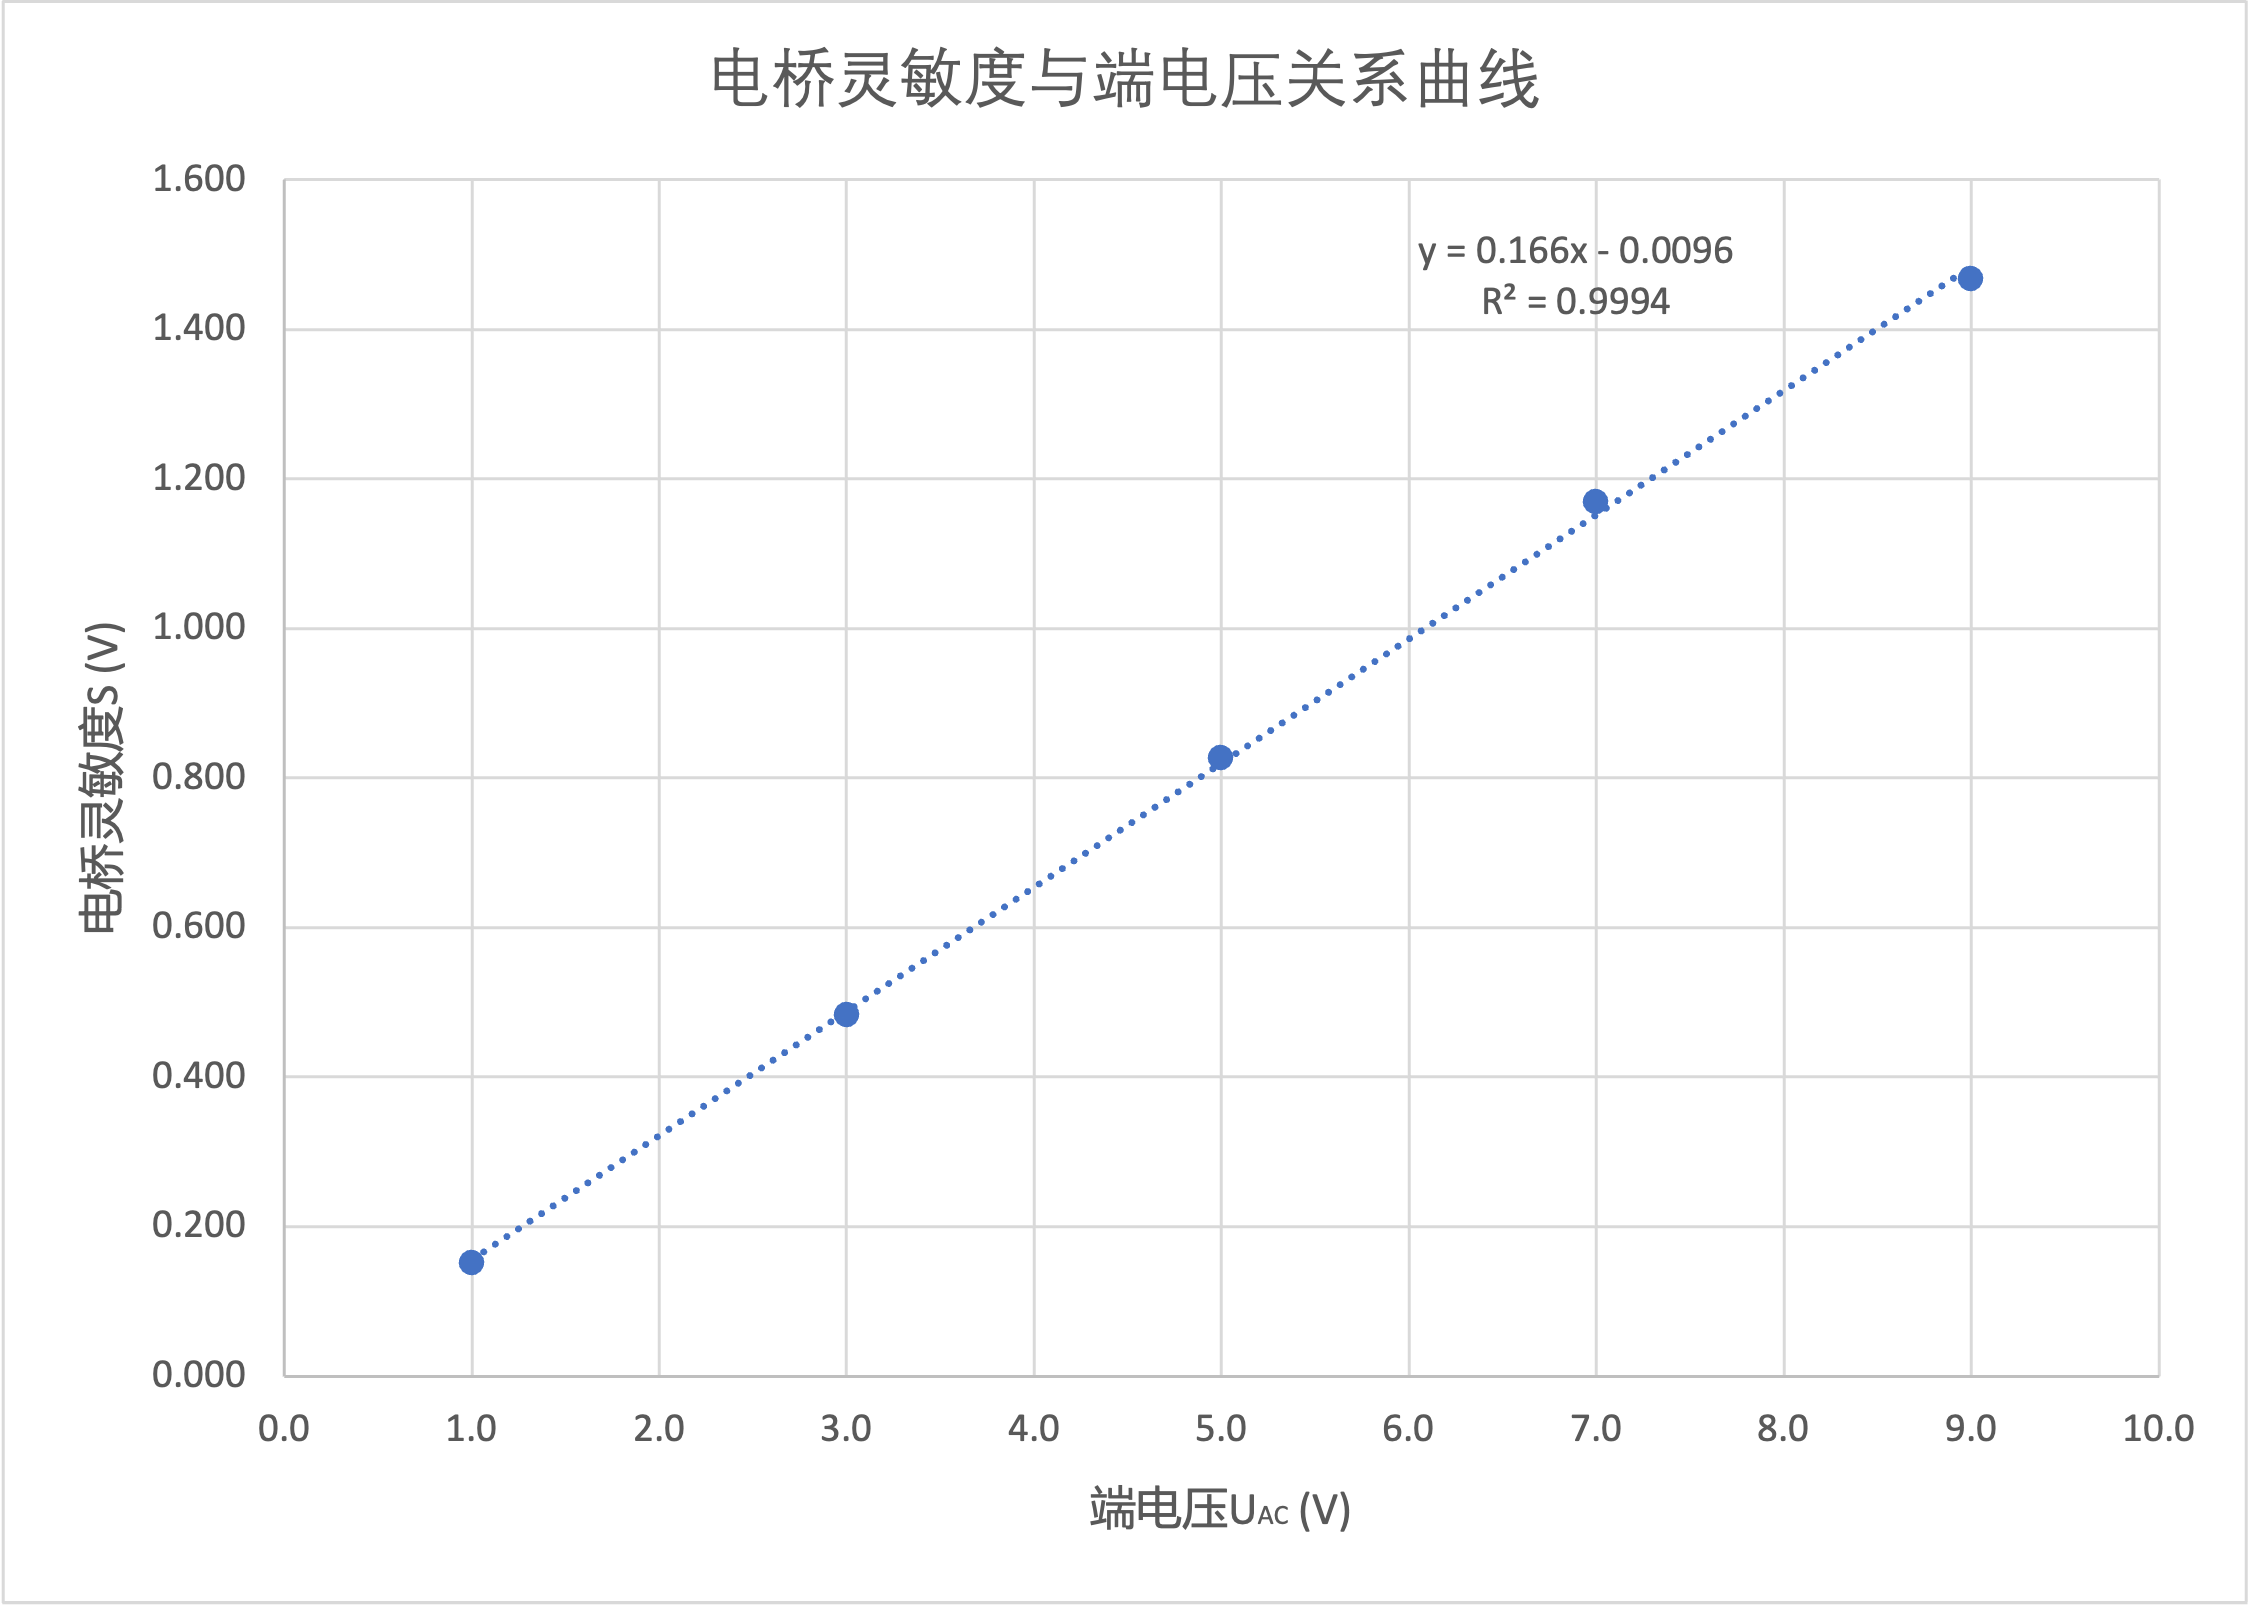
\includegraphics[width=1.0\textwidth]{2-2.png}
    \caption{电桥灵敏度与端电压曲线}
\end{figure*}

线性拟合结果为$y = 0.17x - 0.01, R^2 = 0.9994 > 0.99 $

\newpage

\section{分析与讨论}
1. 从电阻测量结果和万用表测量结果的对比,以及线性拟合的结果判断,本次实验还是较为精确的

2. 本次实验可能的误差来源有:
\begin{itemize}
    \item 电阻臂上的定值电阻并未进行校准,可能存在误差
    \item 由于毫伏表在平衡时并不为0,即使为0,由于实际电阻值和设定有差异,电桥也可能并不平衡
\end{itemize}

3. 若要提高实验的精确度,需要采用更为精确的电阻和测量仪器

\end{document}